\documentclass[11pt, letterpaper]{article}

% Fonts and Encoding
\usepackage[utf8]{inputenc}
\usepackage[T1]{fontenc}
\usepackage{lmodern} % High-quality Latin Modern vector font

% Math and Symbols
\usepackage{amsmath, amssymb, amsthm, amsfonts, mathrsfs, mathtools}

% Layout and Geometry
\usepackage{geometry}
\geometry{letterpaper, margin=1in}
\setlength{\parindent}{0pt}
\setlength{\parskip}{0.6em}

% Formatting and Graphics
\usepackage{graphicx, xcolor, enumitem, booktabs, array, tabularx}

% TikZ for Illustrations
\usepackage{tikz}
\usetikzlibrary{arrows.meta, positioning, shapes.geometric, calc, backgrounds, matrix}

% Clickable Links and TOC
\usepackage{hyperref}
\hypersetup{
    colorlinks=true,
    linkcolor=blue,
    filecolor=magenta,      
    urlcolor=cyan,
    pdftitle={Advanced Mathematics Topic},
}

% Theorem Environments
\newtheorem{theorem}{Theorem}[section]
\newtheorem{lemma}[theorem]{Lemma}
\newtheorem{proposition}[theorem]{Proposition}
\newtheorem{corollary}[theorem]{Corollary}
\theoremstyle{definition}
\newtheorem{definition}{Definition}[section]
\newtheorem{axiom}{Axiom}[section]
\newtheorem{example}{Example}[section]
\theoremstyle{remark}
\newtheorem{remark}{Remark}[section]

% Custom Commands (Enforced standard notation)
\newcommand{\R}{\mathbb{R}}
\newcommand{\N}{\mathbb{N}}
\newcommand{\Z}{\mathbb{Z}}
\newcommand{\Q}{\mathbb{Q}}
\newcommand{\E}{\mathbb{E}}
\newcommand{\Prob}{\mathbb{P}}
\newcommand{\F}{\mathcal{F}}

\title{Series Solutions of Differential Equations: \\ The Taylor Polynomial Approximation}
\author{Tashfeen Omran}
\date{\today}

\begin{document}

\maketitle
\tableofcontents
\newpage

\section{Comprehensive Introduction, Context, and Prerequisites}

\subsection{Core Concepts}
The core objective of this topic is to approximate the solution to a differential equation (DE) near a specific point, $x_0$, using a polynomial. Often, differential equations cannot be solved exactly in terms of elementary functions (like sines, cosines, or exponentials). When an exact analytical solution is impossible, we can construct a \textbf{Taylor Polynomial} that perfectly matches the unknown solution's value and its derivatives at the initial point $x_0$. 

By differentiating the given differential equation repeatedly, we can extract the values of higher-order derivatives of the solution at $x_0$ without ever actually knowing the closed-form solution. These derivatives are then plugged directly into the standard Taylor polynomial formula.

\subsection{Intuition and Derivation}
A Taylor polynomial of degree $n$, denoted $p_n(x)$, is designed to mimic a function $f(x)$ near $x_0$. To make the polynomial behave like $f(x)$, we force it to have the same starting value, the same slope, the same concavity, and so on, up to the $n$-th derivative. 

If we assume $p_n(x) = c_0 + c_1(x-x_0) + c_2(x-x_0)^2 + \dots + c_n(x-x_0)^n$, and we enforce the condition that $p_n^{(j)}(x_0) = f^{(j)}(x_0)$ for all $j \le n$, we find that the coefficients must be $c_j = \frac{f^{(j)}(x_0)}{j!}$. 

In the context of differential equations, the DE itself acts as a "derivative generator." If we are given $y' = F(x, y)$ and an initial condition $y(x_0) = y_0$, we immediately have the first derivative. By applying the chain rule and product rule to differentiate $F(x, y)$ with respect to $x$, we can find $y''$, $y'''$, and so forth, evaluating each at $x_0$.

\subsection{Historical Context and Motivation}
In the 18th and 19th centuries, mathematicians like Leonhard Euler, Joseph-Louis Lagrange, and Brook Taylor were grappling with celestial mechanics and physics problems that yielded complex differential equations. They quickly realized that most DEs do not have neat, closed-form solutions. The Taylor series provided a powerful workaround: if a function is analytic (smooth and well-behaved), it can be entirely reconstructed from the knowledge of its derivatives at a single point. This shifted the paradigm of differential equations from "finding an exact formula" to "constructing an arbitrarily accurate local approximation."

\subsection{Key Formulas}
\begin{itemize}
    \item \textbf{Taylor Polynomial of Degree $n$ centered at $x_0$}:
    \[ p_n(x) = \sum_{j=0}^n \frac{f^{(j)}(x_0)}{j!} (x - x_0)^j = f(x_0) + f'(x_0)(x-x_0) + \frac{f''(x_0)}{2!}(x-x_0)^2 + \dots \]
    \item \textbf{Lagrange Error Bound (Remainder)}:
    \[ \varepsilon_n(x) = f(x) - p_n(x) = \frac{f^{(n+1)}(\xi)}{(n+1)!} (x - x_0)^{n+1} \]
    where $\xi$ is some unknown value strictly between $x_0$ and $x$.
\end{itemize}

\subsection{Prerequisites}
To succeed in this chapter, you must be highly proficient in:
\begin{enumerate}
    \item \textbf{Implicit Differentiation}: Differentiating expressions involving $y$ with respect to $x$, remembering to multiply by $y'$ (Chain Rule).
    \item \textbf{Product and Quotient Rules}: Essential for finding higher-order derivatives of the DE.
    \item \textbf{L'Hôpital's Rule}: Required for resolving indeterminate forms $0/0$ that occasionally appear when evaluating derivatives at singular points.
    \item \textbf{Bounding Functions}: Necessary for the Lagrange Error Bound, specifically finding the maximum value of a derivative on a given interval.
\end{enumerate}

\newpage
\section{Detailed Homework Solutions}

\subsection{Problems 1--8: First Three Nonzero Terms}
\textbf{Instructions:} Determine the first three nonzero terms in the Taylor polynomial approximations for the given initial value problem.

---

\textbf{Problem 1:} $y' = x^2 + y^2 ; \quad y(0) = 1$

\textbf{Solution:}
We need to find the derivatives of $y$ at $x=0$.
\begin{align*}
    y(0) &= 1 \\
    y'(x) &= x^2 + y^2 \implies y'(0) = 0^2 + (1)^2 = 1
\end{align*}
Differentiate $y'$ implicitly with respect to $x$:
\begin{align*}
    y''(x) &= 2x + 2yy' \\
    y''(0) &= 2(0) + 2(1)(1) = 2
\end{align*}
We now have three nonzero derivatives: $y(0)=1$, $y'(0)=1$, and $y''(0)=2$. The Taylor polynomial is:
\[ p_2(x) = y(0) + y'(0)x + \frac{y''(0)}{2!}x^2 = 1 + 1x + \frac{2}{2}x^2 = 1 + x + x^2 \]
\textbf{Final Answer:} The first three nonzero terms are $1, x, x^2$.

---

\textbf{Problem 2:} $y' = y^2 ; \quad y(0) = 2$

\textbf{Solution:}
Evaluate the derivatives at $x=0$:
\begin{align*}
    y(0) &= 2 \\
    y'(x) &= y^2 \implies y'(0) = (2)^2 = 4 \\
    y''(x) &= 2yy' \implies y''(0) = 2(2)(4) = 16
\end{align*}
Construct the polynomial:
\[ p_2(x) = y(0) + y'(0)x + \frac{y''(0)}{2!}x^2 = 2 + 4x + \frac{16}{2}x^2 = 2 + 4x + 8x^2 \]
\textbf{Final Answer:} The first three nonzero terms are $2, 4x, 8x^2$.

---

\textbf{Problem 3:} $y' = \sin y + e^x ; \quad y(0) = 0$

\textbf{Solution:}
Evaluate the derivatives at $x=0$:
\begin{align*}
    y(0) &= 0 \\
    y'(x) &= \sin y + e^x \implies y'(0) = \sin(0) + e^0 = 1 \\
    y''(x) &= y'\cos y + e^x \implies y''(0) = (1)\cos(0) + e^0 = 1 + 1 = 2
\end{align*}
Currently, our terms are $0, 1x, \frac{2}{2}x^2$. We need three \textit{nonzero} terms, so we must find $y'''(0)$.
\begin{align*}
    y'''(x) &= y''\cos y - (y')^2\sin y + e^x \\
    y'''(0) &= (2)\cos(0) - (1)^2\sin(0) + e^0 = 2 - 0 + 1 = 3
\end{align*}
Construct the polynomial:
\[ p_3(x) = 0 + 1x + \frac{2}{2!}x^2 + \frac{3}{3!}x^3 = x + x^2 + \frac{1}{2}x^3 \]
\textbf{Final Answer:} The first three nonzero terms are $x, x^2, \frac{1}{2}x^3$.

---

\textbf{Problem 4:} $y' = \sin(x+y) ; \quad y(0) = 0$

\textbf{Solution:}
Evaluate the derivatives at $x=0$:
\begin{align*}
    y(0) &= 0 \\
    y'(x) &= \sin(x+y) \implies y'(0) = \sin(0+0) = 0 \\
    y''(x) &= (1+y')\cos(x+y) \implies y''(0) = (1+0)\cos(0) = 1 \\
    y'''(x) &= y''\cos(x+y) - (1+y')^2\sin(x+y) \implies y'''(0) = (1)(1) - (1)^2(0) = 1
\end{align*}
So far, the nonzero terms are $\frac{1}{2}x^2$ and $\frac{1}{6}x^3$. We need one more.
\begin{align*}
    y^{(4)}(x) &= y'''\cos(x+y) - y''(1+y')\sin(x+y) - 2(1+y')y''\sin(x+y) - (1+y')^3\cos(x+y) \\
    y^{(4)}(0) &= (1)(1) - (1)(1)(0) - 2(1)(1)(0) - (1)^3(1) = 1 - 1 = 0
\end{align*}
We must go to the fifth derivative. To simplify, note that at $x=0$, $\sin(x+y)=0$ and $\cos(x+y)=1$.
\begin{align*}
    y^{(5)}(x) &= y^{(4)}\cos(x+y) - y'''(1+y')\sin(x+y) \\
    &\quad - 3(y'')^2\sin(x+y) - 3(1+y')y'''\sin(x+y) - 3(1+y')^2 y''\cos(x+y) \\
    &\quad + (1+y')^4\sin(x+y) \\
    y^{(5)}(0) &= (0)(1) - 0 - 0 - 0 - 3(1)^2(1)(1) + 0 = -3
\end{align*}
Construct the polynomial:
\[ p_5(x) = \frac{1}{2!}x^2 + \frac{1}{3!}x^3 - \frac{3}{5!}x^5 = \frac{1}{2}x^2 + \frac{1}{6}x^3 - \frac{1}{40}x^5 \]
\textbf{Final Answer:} The first three nonzero terms are $\frac{1}{2}x^2, \frac{1}{6}x^3, -\frac{1}{40}x^5$.

---

\textbf{Problem 5:} $x'' + tx = 0 ; \quad x(0) = 1 , \quad x'(0) = 0$

\textbf{Solution:}
Here, $x$ is the dependent variable and $t$ is the independent variable. We rewrite the DE as $x''(t) = -tx(t)$.
\begin{align*}
    x(0) &= 1 \\
    x'(0) &= 0 \\
    x''(t) &= -tx(t) \implies x''(0) = 0 \\
    x'''(t) &= -x(t) - tx'(t) \implies x'''(0) = -1 - 0 = -1 \\
    x^{(4)}(t) &= -x'(t) - x'(t) - tx''(t) = -2x'(t) - tx''(t) \implies x^{(4)}(0) = 0 \\
    x^{(5)}(t) &= -2x''(t) - x''(t) - tx'''(t) = -3x''(t) - tx'''(t) \implies x^{(5)}(0) = 0 \\
    x^{(6)}(t) &= -3x'''(t) - x'''(t) - tx^{(4)}(t) = -4x'''(t) - tx^{(4)}(t) \implies x^{(6)}(0) = -4(-1) - 0 = 4
\end{align*}
The nonzero derivatives are $x(0)=1$, $x'''(0)=-1$, and $x^{(6)}(0)=4$.
\[ p_6(t) = 1 - \frac{1}{3!}t^3 + \frac{4}{6!}t^6 = 1 - \frac{1}{6}t^3 + \frac{4}{720}t^6 = 1 - \frac{1}{6}t^3 + \frac{1}{180}t^6 \]
\textbf{Final Answer:} The first three nonzero terms are $1, -\frac{1}{6}t^3, \frac{1}{180}t^6$.

---

\textbf{Problem 6:} $y'' + y = 0 ; \quad y(0) = 0 , \quad y'(0) = 1$

\textbf{Solution:}
Rewrite as $y'' = -y$.
\begin{align*}
    y(0) &= 0 \\
    y'(0) &= 1 \\
    y''(0) &= -y(0) = 0 \\
    y'''(0) &= -y'(0) = -1 \\
    y^{(4)}(0) &= -y''(0) = 0 \\
    y^{(5)}(0) &= -y'''(0) = 1
\end{align*}
The nonzero derivatives are $y'(0)=1$, $y'''(0)=-1$, and $y^{(5)}(0)=1$.
\[ p_5(x) = 1x - \frac{1}{3!}x^3 + \frac{1}{5!}x^5 = x - \frac{1}{6}x^3 + \frac{1}{120}x^5 \]
\textbf{Final Answer:} The first three nonzero terms are $x, -\frac{1}{6}x^3, \frac{1}{120}x^5$.

---

\textbf{Problem 7:} $y''(\theta) + y(\theta)^3 = \sin\theta ; \quad y(0) = 0 , \quad y'(0) = 0$

\textbf{Solution:}
Rewrite as $y'' = \sin\theta - y^3$.
\begin{align*}
    y(0) &= 0 \\
    y'(0) &= 0 \\
    y''(0) &= \sin(0) - 0^3 = 0 \\
    y'''(\theta) &= \cos\theta - 3y^2 y' \implies y'''(0) = 1 - 0 = 1 \\
    y^{(4)}(\theta) &= -\sin\theta - 6y(y')^2 - 3y^2 y'' \implies y^{(4)}(0) = 0 - 0 - 0 = 0 \\
    y^{(5)}(\theta) &= -\cos\theta - 6(y')^3 - 12yy'y'' - 6yy'y'' - 3y^2 y''' \implies y^{(5)}(0) = -1 - 0 = -1
\end{align*}
We need one more nonzero term. Notice that any term containing $y$ or $y'$ will evaluate to 0 at $\theta=0$.
\begin{align*}
    y^{(6)}(\theta) &= \sin\theta - 18(y')^2 y'' - \dots \text{(all terms contain } y \text{ or } y') \implies y^{(6)}(0) = 0 \\
    y^{(7)}(\theta) &= \cos\theta - 36y'(y'')^2 - 18(y')^2 y''' - \dots \implies y^{(7)}(0) = 1
\end{align*}
The nonzero derivatives are $y'''(0)=1$, $y^{(5)}(0)=-1$, and $y^{(7)}(0)=1$.
\[ p_7(\theta) = \frac{1}{3!}\theta^3 - \frac{1}{5!}\theta^5 + \frac{1}{7!}\theta^7 = \frac{1}{6}\theta^3 - \frac{1}{120}\theta^5 + \frac{1}{5040}\theta^7 \]
\textbf{Final Answer:} The first three nonzero terms are $\frac{1}{6}\theta^3, -\frac{1}{120}\theta^5, \frac{1}{5040}\theta^7$.

---

\textbf{Problem 8:} $y'' + \sin y = 0 ; \quad y(0) = 1 , \quad y'(0) = 0$

\textbf{Solution:}
Rewrite as $y'' = -\sin y$.
\begin{align*}
    y(0) &= 1 \\
    y'(0) &= 0 \\
    y''(0) &= -\sin(1) \\
    y'''(x) &= -y'\cos y \implies y'''(0) = -(0)\cos(1) = 0 \\
    y^{(4)}(x) &= -y''\cos y + (y')^2\sin y \implies y^{(4)}(0) = -(-\sin 1)\cos 1 + 0 = \sin 1 \cos 1
\end{align*}
The nonzero derivatives are $y(0)=1$, $y''(0)=-\sin 1$, and $y^{(4)}(0)=\sin 1 \cos 1$.
\[ p_4(x) = 1 - \frac{\sin 1}{2!}x^2 + \frac{\sin 1 \cos 1}{4!}x^4 = 1 - \frac{\sin 1}{2}x^2 + \frac{\sin 1 \cos 1}{24}x^4 \]
\textbf{Final Answer:} The first three nonzero terms are $1, -\frac{\sin 1}{2}x^2, \frac{\sin 1 \cos 1}{24}x^4$.

---

\subsection{Problems 9--10: Error Bounding}

\textbf{Problem 9:} 
(a) Construct the Taylor polynomial $p_3(x)$ of degree 3 for $f(x) = \ln x$ around $x = 1$. \\
(b) Using the error formula, show that $|\ln(1.5) - p_3(1.5)| \le \frac{(0.5)^4}{4} = 0.015625$. \\
(c) Compare the estimate in part (b) with the actual error. \\
(d) Sketch the graphs of $\ln x$ and $p_3(x)$ for $0 < x < 2$.

\textbf{Solution:}
\textbf{Part (a):}
\begin{align*}
    f(x) &= \ln x \implies f(1) = 0 \\
    f'(x) &= x^{-1} \implies f'(1) = 1 \\
    f''(x) &= -x^{-2} \implies f''(1) = -1 \\
    f'''(x) &= 2x^{-3} \implies f'''(1) = 2
\end{align*}
\[ p_3(x) = 0 + 1(x-1) - \frac{1}{2!}(x-1)^2 + \frac{2}{3!}(x-1)^3 = (x-1) - \frac{1}{2}(x-1)^2 + \frac{1}{3}(x-1)^3 \]

\textbf{Part (b):}
The Lagrange error bound is $\varepsilon_3(x) = \frac{f^{(4)}(\xi)}{4!}(x-1)^4$, where $\xi$ is between $1$ and $x$.
\[ f^{(4)}(x) = -6x^{-4} \]
At $x = 1.5$, $\xi \in (1, 1.5)$.
\[ |\varepsilon_3(1.5)| = \left| \frac{-6\xi^{-4}}{24} (1.5 - 1)^4 \right| = \frac{1}{4\xi^4} (0.5)^4 \]
To maximize this error, we must minimize the denominator $\xi^4$ on the interval $(1, 1.5)$. The minimum value of $\xi$ is $1$.
\[ |\varepsilon_3(1.5)| \le \frac{1}{4(1)^4} (0.5)^4 = \frac{(0.5)^4}{4} = 0.015625 \]

\textbf{Part (c):}
Actual value: $p_3(1.5) = (0.5) - \frac{1}{2}(0.25) + \frac{1}{3}(0.125) = 0.5 - 0.125 + 0.041667 = 0.416667$.
The true value is $\ln(1.5) \approx 0.405465$.
Actual error $= |0.405465 - 0.416667| = 0.011202$.
The actual error ($0.011202$) is indeed less than the theoretical maximum bound ($0.015625$).

\textbf{Part (d):}
\begin{center}
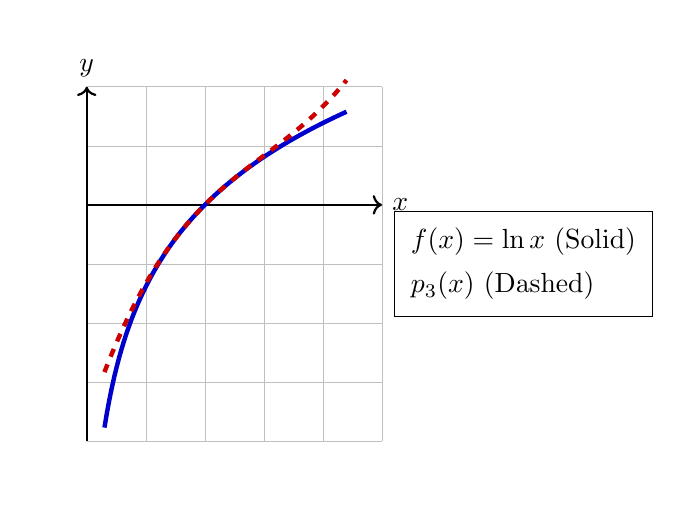
\begin{tikzpicture}[scale=1.5]
    \fill[white] (-0.5, -2.5) rectangle (3.5, 1.5);
    \draw[lightgray, very thin, step=0.5] (0,-2) grid (2.5,1);
    \draw[->, thick] (0,0) -- (2.5,0) node[right] {$x$};
    \draw[->, thick] (0,-2) -- (0,1) node[above] {$y$};
    
    % Plot ln(x)
    \draw[ultra thick, blue!80!black, domain=0.15:2.2, samples=100] plot (\x, {ln(\x)});
    
    % Plot p_3(x)
    \draw[ultra thick, red!80!black, dashed, domain=0.15:2.2, samples=100] plot (\x, {(\x-1) - 0.5*(\x-1)^2 + 0.3333*(\x-1)^3});
    
    % Legend
    \node[align=left, fill=white, draw=black, inner sep=6pt, anchor=west] at (2.6, -0.5) {
        $\displaystyle f(x) = \ln x$ (Solid) \\[4pt]
        $\displaystyle p_3(x)$ (Dashed)
    };
\end{tikzpicture}
\end{center}

---

\textbf{Problem 10:} 
(a) Construct the Taylor polynomial $p_3(x)$ of degree 3 for $f(x) = 1/(2-x)$ around $x = 0$. \\
(b) Using the error formula, show that $|f(1/2) - p_3(1/2)| \le \frac{2}{3^5}$. \\
(c) Compare the estimate in part (b) with the actual error. \\
(d) Sketch the graphs for $-2 < x < 2$.

\textbf{Solution:}
\textbf{Part (a):}
\begin{align*}
    f(x) &= (2-x)^{-1} \implies f(0) = \frac{1}{2} \\
    f'(x) &= (2-x)^{-2} \implies f'(0) = \frac{1}{4} \\
    f''(x) &= 2(2-x)^{-3} \implies f''(0) = \frac{2}{8} = \frac{1}{4} \\
    f'''(x) &= 6(2-x)^{-4} \implies f'''(0) = \frac{6}{16} = \frac{3}{8}
\end{align*}
\[ p_3(x) = \frac{1}{2} + \frac{1}{4}x + \frac{1/4}{2!}x^2 + \frac{3/8}{3!}x^3 = \frac{1}{2} + \frac{1}{4}x + \frac{1}{8}x^2 + \frac{1}{16}x^3 \]

\textbf{Part (b):}
The error bound is $\varepsilon_3(x) = \frac{f^{(4)}(\xi)}{4!}x^4$.
\[ f^{(4)}(x) = 24(2-x)^{-5} \]
At $x = 1/2$, $\xi \in (0, 1/2)$.
\[ |\varepsilon_3(1/2)| = \left| \frac{24(2-\xi)^{-5}}{24} \left(\frac{1}{2}\right)^4 \right| = \frac{1}{16(2-\xi)^5} \]
To maximize this, we minimize the denominator by choosing the largest $\xi$ in the interval, which is $\xi = 1/2$.
\[ |\varepsilon_3(1/2)| \le \frac{1}{16(2 - 0.5)^5} = \frac{1}{16(3/2)^5} = \frac{32}{16 \cdot 243} = \frac{2}{243} = \frac{2}{3^5} \]

\textbf{Part (c):}
Actual value: $f(1/2) = \frac{1}{2 - 0.5} = \frac{1}{1.5} = \frac{2}{3} = \frac{256}{384}$.
Polynomial value: $p_3(1/2) = \frac{1}{2} + \frac{1}{8} + \frac{1}{32} + \frac{1}{128} = \frac{64 + 16 + 4 + 1}{128} = \frac{85}{128} = \frac{255}{384}$.
Actual error $= \left| \frac{256}{384} - \frac{255}{384} \right| = \frac{1}{384}$.
Comparing them: $\frac{1}{384} \approx 0.00260$ and $\frac{2}{243} \approx 0.00823$. The actual error is well within the bound.

\textbf{Part (d):}
\begin{center}
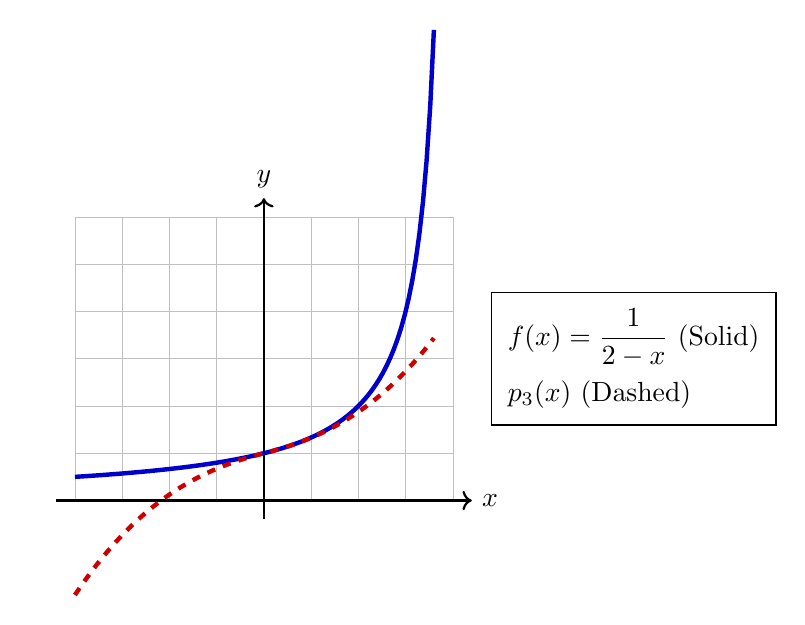
\begin{tikzpicture}[scale=1.2]
    \fill[white] (-2.5, -0.5) rectangle (3.5, 3.5);
    \draw[lightgray, very thin, step=0.5] (-2,0) grid (2,3);
    \draw[->, thick] (-2.2,0) -- (2.2,0) node[right] {$x$};
    \draw[->, thick] (0,-0.2) -- (0,3.2) node[above] {$y$};
    
    % Plot 1/(2-x)
    \draw[ultra thick, blue!80!black, domain=-2:1.8, samples=100] plot (\x, {1/(2-\x)});
    
    % Plot p_3(x)
    \draw[ultra thick, red!80!black, dashed, domain=-2:1.8, samples=100] plot (\x, {0.5 + 0.25*\x + 0.125*\x^2 + 0.0625*\x^3});
    
    % Legend
    \node[align=left, fill=white, draw=black, inner sep=6pt, anchor=west] at (2.4, 1.5) {
        $\displaystyle f(x) = \frac{1}{2-x}$ (Solid) \\[4pt]
        $\displaystyle p_3(x)$ (Dashed)
    };
\end{tikzpicture}
\end{center}

---

\subsection{Problems 11--12: Theoretical Proofs}

\textbf{Problem 11:} Argue that if $y = \phi(x)$ is a solution to $y'' + p(x)y' + q(x)y = g(x)$ on $(a, b)$, where $p, q, g$ are twice-differentiable, then the fourth derivative of $\phi(x)$ exists on $(a, b)$.

\textbf{Solution:}
Since $y$ is a solution to the second-order DE, $y$ and $y'$ must exist and be continuous. We can isolate $y''$:
\[ y'' = g(x) - p(x)y' - q(x)y \]
Because $p, q, g$ are twice-differentiable, they are continuous. Since $y, y'$ are continuous, the right side is continuous, meaning $y''$ is continuous.
Differentiating both sides with respect to $x$:
\[ y''' = g'(x) - p'(x)y' - p(x)y'' - q'(x)y - q(x)y' \]
Since $p, q, g$ are twice-differentiable, $p', q', g'$ exist. We already established $y, y', y''$ exist. Therefore, $y'''$ exists.
Differentiating again:
\[ y^{(4)} = g''(x) - p''(x)y' - 2p'(x)y'' - p(x)y''' - q''(x)y - 2q'(x)y' - q(x)y'' \]
Since $p, q, g$ are twice-differentiable, $p'', q'', g''$ exist. We just proved $y'''$ exists. Thus, every term on the right side exists, proving that $y^{(4)}$ exists on $(a, b)$.

---

\textbf{Problem 12:} Argue that if $p, q, g$ possess derivatives of all orders, then $\phi$ has derivatives of all orders.

\textbf{Solution:}
We proceed by mathematical induction. 
\textbf{Base Case:} $y'' = g(x) - p(x)y' - q(x)y$. Since $p, q, g, y, y'$ exist, $y''$ exists.
\textbf{Inductive Step:} Assume that $y^{(k)}$ exists for all $k \le n$. We want to show $y^{(n+1)}$ exists.
We know $y^{(n)} = \frac{d^{n-2}}{dx^{n-2}} [g(x) - p(x)y' - q(x)y]$.
By the generalized Leibniz rule for differentiation, the $(n-2)$-th derivative of a product like $p(x)y'$ is a linear combination of products of the derivatives of $p(x)$ (up to order $n-2$) and derivatives of $y'$ (up to order $n-2$, which is $y^{(n-1)}$).
Since $p, q, g$ have derivatives of all orders, their derivatives always exist. By our inductive hypothesis, all derivatives of $y$ up to order $n$ exist. Therefore, we can differentiate $y^{(n)}$ one more time to get $y^{(n+1)}$, which will depend only on derivatives of $p, q, g$ (which exist) and derivatives of $y$ up to order $n$ (which exist). Thus, $\phi$ has derivatives of all orders.

---

\subsection{Problems 13--14: Duffing's Equation}

\textbf{Problem 13:} $y'' + ky + ry^3 = A\cos(\omega t)$. Let $k=r=A=1, \omega=10$. Find the first three nonzero terms for $y(0)=0, y'(0)=1$.

\textbf{Solution:}
The equation is $y'' + y + y^3 = \cos(10t)$.
\begin{align*}
    y(0) &= 0 \\
    y'(0) &= 1 \\
    y''(0) &= \cos(0) - y(0) - y(0)^3 = 1 - 0 - 0 = 1 \\
    y'''(t) &= -10\sin(10t) - y' - 3y^2 y' \implies y'''(0) = 0 - 1 - 0 = -1
\end{align*}
The first three nonzero derivatives are $y'(0)=1$, $y''(0)=1$, and $y'''(0)=-1$.
\[ p_3(t) = 0 + 1t + \frac{1}{2!}t^2 - \frac{1}{3!}t^3 = t + \frac{1}{2}t^2 - \frac{1}{6}t^3 \]
\textbf{Final Answer:} The first three nonzero terms are $t, \frac{1}{2}t^2, -\frac{1}{6}t^3$.

---

\textbf{Problem 14:} Soft vs Hard Springs.
(a) Redo Problem 13 with $r = -1$.
(b) Keep $k=A=1, \omega=10$, change to $y(0)=1, y'(0)=0$. Redo with $r = \pm 1$.
(c) Is there a difference between soft and hard springs for small $t$?

\textbf{Solution:}
\textbf{Part (a):} $r = -1 \implies y'' + y - y^3 = \cos(10t)$. $y(0)=0, y'(0)=1$.
\begin{align*}
    y''(0) &= \cos(0) - y(0) + y(0)^3 = 1 - 0 + 0 = 1 \\
    y'''(t) &= -10\sin(10t) - y' + 3y^2 y' \implies y'''(0) = 0 - 1 + 0 = -1
\end{align*}
The polynomial is $t + \frac{1}{2}t^2 - \frac{1}{6}t^3$. It is identical to Problem 13 for small $t$.

\textbf{Part (b):} $y(0)=1, y'(0)=0$.
\textit{Hard Spring ($r=1$):} $y'' + y + y^3 = \cos(10t)$.
\begin{align*}
    y''(0) &= 1 - 1 - 1^3 = -1 \\
    y'''(t) &= -10\sin(10t) - y' - 3y^2 y' \implies y'''(0) = 0 - 0 - 0 = 0 \\
    y^{(4)}(t) &= -100\cos(10t) - y'' - 6y(y')^2 - 3y^2 y'' \\
    y^{(4)}(0) &= -100 - (-1) - 0 - 3(1)^2(-1) = -100 + 1 + 3 = -96
\end{align*}
Terms: $1, -\frac{1}{2}t^2, -\frac{96}{24}t^4 = -4t^4$.

\textit{Soft Spring ($r=-1$):} $y'' + y - y^3 = \cos(10t)$.
\begin{align*}
    y''(0) &= 1 - 1 + 1^3 = 1 \\
    y'''(t) &= -10\sin(10t) - y' + 3y^2 y' \implies y'''(0) = 0 - 0 + 0 = 0 \\
    y^{(4)}(t) &= -100\cos(10t) - y'' + 6y(y')^2 + 3y^2 y'' \\
    y^{(4)}(0) &= -100 - (1) + 0 + 3(1)^2(1) = -100 - 1 + 3 = -98
\end{align*}
Terms: $1, \frac{1}{2}t^2, -\frac{98}{24}t^4 = -\frac{49}{12}t^4$.

\textbf{Part (c):} Yes, there is a massive difference. For the hard spring, $y''(0) = -1$, meaning the spring immediately accelerates back toward the equilibrium position (strong restoring force). For the soft spring, $y''(0) = 1$, meaning the spring initially accelerates \textit{away} from equilibrium because the external forcing function overpowers the weak restoring force.

---

\subsection{Problems 15--16: Advanced Equations}

\textbf{Problem 15:} $xy'' + 2y' + xy = 0 ; \quad y(0) = 1 , \quad y'(0) = 0$. Use L'Hôpital's rule to compute $p_2(x)$.

\textbf{Solution:}
Isolating $y''$ gives $y'' = \frac{-2y' - xy}{x}$. At $x=0$, this evaluates to $\frac{0}{0}$.
We apply L'Hôpital's rule by differentiating the numerator and denominator with respect to $x$:
\[ \lim_{x \to 0} y''(x) = \lim_{x \to 0} \frac{\frac{d}{dx}[-2y' - xy]}{\frac{d}{dx}[x]} = \lim_{x \to 0} \frac{-2y'' - (y + xy')}{1} \]
Assuming $y''$ is continuous at $0$, we can set $y''(0)$ equal to this limit:
\begin{align*}
    y''(0) &= -2y''(0) - y(0) - 0 \cdot y'(0) \\
    y''(0) &= -2y''(0) - 1 \\
    3y''(0) &= -1 \implies y''(0) = -\frac{1}{3}
\end{align*}
The Taylor polynomial of degree 2 is:
\[ p_2(x) = y(0) + y'(0)x + \frac{y''(0)}{2}x^2 = 1 + 0x - \frac{1/3}{2}x^2 = 1 - \frac{1}{6}x^2 \]
\textbf{Final Answer:} $p_2(x) = 1 - \frac{1}{6}x^2$.

---

\textbf{Problem 16:} van der Pol Equation: $y'' + 0.1(y^2 - 1)y' + y = 0 ; \quad y(0) = 1 , \quad y'(0) = 0$. Find $p_4(x)$.

\textbf{Solution:}
Rewrite as $y'' = -0.1(y^2 - 1)y' - y$.
\begin{align*}
    y(0) &= 1 \\
    y'(0) &= 0 \\
    y''(0) &= -0.1(1^2 - 1)(0) - 1 = -1 \\
    y'''(x) &= -0.1[2yy'(y') + (y^2 - 1)y''] - y' = -0.2y(y')^2 - 0.1(y^2 - 1)y'' - y' \\
    y'''(0) &= -0.2(1)(0)^2 - 0.1(0)(-1) - 0 = 0 \\
    y^{(4)}(x) &= -0.2[(y')^3 + 2yy'y''] - 0.1[2yy'y'' + (y^2 - 1)y'''] - y'' \\
    y^{(4)}(0) &= -0.2[0 + 0] - 0.1[0 + 0] - (-1) = 1
\end{align*}
Construct the polynomial:
\[ p_4(x) = 1 + 0x - \frac{1}{2!}x^2 + \frac{0}{3!}x^3 + \frac{1}{4!}x^4 = 1 - \frac{1}{2}x^2 + \frac{1}{24}x^4 \]
\textbf{Final Answer:} $p_4(x) = 1 - \frac{1}{2}x^2 + \frac{1}{24}x^4$.

\newpage
\section{In-Depth Analysis of Problems and Techniques}

\subsection{A) Problem Types and General Approach}
\begin{itemize}
    \item \textbf{Type 1: Direct Initial Value Problems (Problems 1-8, 13-14, 16)}
    \textit{Strategy:} Isolate the highest derivative on one side of the equation. Plug in the initial conditions to find its value. Then, implicitly differentiate the entire equation with respect to the independent variable to generate formulas for higher-order derivatives.
    
    \item \textbf{Type 2: Error Bounding / Lagrange Remainder (Problems 9-10)}
    \textit{Strategy:} Calculate the $(n+1)$-th derivative of the exact function. Set up the Lagrange error formula. To find the maximum possible error, analyze the $(n+1)$-th derivative on the interval between $x_0$ and the evaluation point $x$, and find the value of $\xi$ that maximizes the absolute value of the expression.
    
    \item \textbf{Type 3: Singular Differential Equations (Problem 15)}
    \textit{Strategy:} When isolating the highest derivative results in division by zero at the initial point (an indeterminate form $0/0$), apply L'Hôpital's rule directly to the differential equation. This creates an algebraic equation where you can solve for the unknown derivative.
\end{itemize}

\subsection{B) Key Algebraic and Calculus Manipulations}
\begin{itemize}
    \item \textbf{Implicit Chain Rule:} Used extensively. For example, in Problem 2, differentiating $y^2$ with respect to $x$ yields $2yy'$. Forgetting the $y'$ is the most common fatal error in this chapter.
    \item \textbf{Product Rule Expansion:} In Problem 4, differentiating $(1+y')\cos(x+y)$ requires careful application of the product rule: $y''\cos(x+y) - (1+y')^2\sin(x+y)$.
    \item \textbf{Zero-Term Elimination:} In Problem 7, recognizing that any term multiplied by $y$ or $y'$ will evaluate to zero at $\theta=0$ saves massive amounts of algebraic expansion time for the 6th and 7th derivatives.
    \item \textbf{Maximizing Rational Functions:} In Problem 10, to maximize $\frac{1}{(2-\xi)^5}$ on $(0, 0.5)$, we must \textit{minimize} the denominator. The denominator is minimized when $\xi$ is as large as possible ($\xi = 0.5$).
\end{itemize}

\section{"Cheatsheet" and Tips for Success}

\renewcommand{\arraystretch}{1.5}
\begin{tabularx}{\textwidth}{l X}
\toprule
\textbf{Concept} & \textbf{Formula / Rule} \\
\midrule
Taylor Polynomial & $\displaystyle p_n(x) = \sum_{j=0}^n \frac{f^{(j)}(x_0)}{j!} (x - x_0)^j$ \\
Lagrange Error & $\displaystyle \varepsilon_n(x) = \frac{f^{(n+1)}(\xi)}{(n+1)!} (x - x_0)^{n+1}$ \\
\bottomrule
\end{tabularx}

\textbf{Top Tricks and Shortcuts:}
\begin{enumerate}
    \item \textbf{Don't simplify the algebra, just plug in the numbers:} When finding $y^{(4)}$ or $y^{(5)}$, do not try to algebraically simplify the massive expression. Immediately plug in $x=0, y=y_0, y'=y'_0$. Most terms will instantly vanish.
    \item \textbf{Watch the wording:} "First three \textit{nonzero} terms" is not the same as "Taylor polynomial of degree 2". If $y'(0)=0$, you might have to calculate up to the 4th or 5th derivative to find three terms that don't vanish.
\end{enumerate}

\textbf{Common Pitfalls:}
\begin{itemize}
    \item \textbf{The Factorial Trap:} Forgetting to divide the $n$-th derivative by $n!$ when assembling the final polynomial.
    \item \textbf{The $\xi$ Trap:} In the Lagrange error bound, $\xi$ is NOT the evaluation point $x$, nor is it the center $x_0$. It is the value \textit{between} them that makes the derivative largest.
\end{itemize}

\newpage
\section{Conceptual Synthesis and The "Big Picture"}

\subsection{A) Thematic Connections}
The central theme of this topic is \textbf{Local Approximation}. We are trading global exactness for local simplicity. This is the exact same philosophy behind the Tangent Line Approximation (Euler's Method) learned in Calculus I. In fact, Euler's Method is simply a Taylor polynomial of degree 1. By adding more terms (degree 2, 3, 4...), we are upgrading our linear approximation to a parabolic, cubic, and quartic approximation, allowing us to take larger steps away from $x_0$ with less error.

\subsection{B) Forward and Backward Links}
\textbf{Backward:} This topic relies heavily on the Taylor Series concepts from Calculus II, but applies them in a reverse-engineered way. Instead of having a function and finding its series, we have a rule (the DE) and we build the function from scratch.
\textbf{Forward:} This is the gateway to the \textbf{Method of Frobenius} and full Power Series Solutions. Instead of stopping at degree $n$, we will soon assume the solution is an infinite series $y = \sum a_n x^n$, plug the entire infinite series into the DE, and solve for a recurrence relation that defines every coefficient simultaneously.

\section{Abstract Real-World Modeling (AI, ML, \& Quant Finance)}

\subsection{A) Concrete Scenarios}
\begin{enumerate}
    \item \textbf{Quantitative Finance (Option Pricing):} In stochastic volatility models (like the Heston model), the differential equations governing the price of an option do not always have closed-form solutions. Quants use Taylor expansions of the drift and diffusion terms (known as the Kramer-Moyal expansion or Ito-Taylor expansion) to approximate the transition probability densities of the underlying assets.
    \item \textbf{Machine Learning (Optimization):} Second-order optimization algorithms, like Newton's Method, rely on a 2nd-degree Taylor polynomial approximation of the Loss function. The algorithm calculates the gradient (1st derivative) and the Hessian matrix (2nd derivative) to find the minimum of the approximating parabola, taking a step in that direction.
\end{enumerate}

\subsection{B) Model Problem Setup: Ito-Taylor Expansion in Stochastic Calculus}
In algorithmic trading, suppose an asset price $X_t$ follows a stochastic differential equation (SDE) driven by a Wiener process $W_t$:
\[ dX_t = a(X_t)dt + b(X_t)dW_t \]
To simulate this path on a computer, we cannot solve it exactly. We use the \textbf{Milstein Scheme}, which is derived via a stochastic Taylor expansion (Ito-Taylor expansion). 
By applying Ito's Lemma to the diffusion term $b(X_t)$, we expand the function to the second order. The resulting discrete-time approximation for a time step $\Delta t$ is:
\[ X_{t+\Delta t} \approx X_t + a(X_t)\Delta t + b(X_t)\Delta W_t + \frac{1}{2} b(X_t) b'(X_t) \left( (\Delta W_t)^2 - \Delta t \right) \]
Here, the term $\frac{1}{2} b(X_t) b'(X_t)$ is the direct stochastic equivalent of the $\frac{y''(0)}{2!}x^2$ term in our deterministic Taylor polynomials, correcting the curvature of the random walk.

\newpage
\section{Common Variations and Untested Concepts}

\textbf{Variation 1: Expansion around $x_0 \neq 0$}
Most homework problems centered the expansion at $x=0$ (Maclaurin series). You must be prepared to expand around $x_0 = c$.
\textit{Example:} $y' = x + y, \quad y(1) = 2$. Find $p_2(x)$ around $x=1$.
\textit{Solution:} 
$y(1) = 2$. 
$y'(1) = 1 + y(1) = 1 + 2 = 3$.
$y'' = 1 + y' \implies y''(1) = 1 + 3 = 4$.
$p_2(x) = 2 + 3(x-1) + \frac{4}{2}(x-1)^2 = 2 + 3(x-1) + 2(x-1)^2$.

\textbf{Variation 2: Systems of Differential Equations}
You may be given two coupled equations.
\textit{Example:} $x' = x + y, \quad y' = x - y$, with $x(0)=1, y(0)=0$. Find the 2nd degree Taylor polynomial for $x(t)$.
\textit{Solution:}
$x(0) = 1$.
$x'(0) = x(0) + y(0) = 1 + 0 = 1$.
$x''(t) = x'(t) + y'(t) = (x+y) + (x-y) = 2x$.
$x''(0) = 2(1) = 2$.
$p_2(t) = 1 + t + t^2$.

\section{Advanced Diagnostic Testing: "Find the Flaw"}

Below are five problems with solutions that contain a subtle, critical flaw. Your task is to act as the grader, find the error, explain it, and correct it.

\textbf{Problem 1:} Find the degree 2 Taylor polynomial for $y' = y^2 + x, y(0)=1$.
\textit{Flawed Solution:} $y(0)=1$. $y'(0) = 1^2 + 0 = 1$. $y'' = 2y + 1 \implies y''(0) = 2(1)+1 = 3$. $p_2(x) = 1 + x + 3x^2$.
\textit{Flaw:} The implicit derivative of $y^2$ is $2yy'$, not $2y$. Also, the factorial was forgotten in the final polynomial.
\textit{Correction:} $y'' = 2yy' + 1 \implies y''(0) = 2(1)(1) + 1 = 3$. $p_2(x) = 1 + x + \frac{3}{2}x^2$.

\textbf{Problem 2:} Find the degree 3 Taylor polynomial for $y' = e^y, y(0)=0$.
\textit{Flawed Solution:} $y(0)=0$. $y'(0) = e^0 = 1$. $y'' = e^y \implies y''(0) = 1$. $y''' = e^y \implies y'''(0) = 1$. $p_3(x) = x + \frac{1}{2}x^2 + \frac{1}{6}x^3$.
\textit{Flaw:} The chain rule was omitted. $y'' = e^y \cdot y'$.
\textit{Correction:} $y'' = e^y y' \implies y''(0) = 1(1) = 1$. $y''' = e^y(y')^2 + e^y y'' \implies y'''(0) = 1(1)^2 + 1(1) = 2$. $p_3(x) = x + \frac{1}{2}x^2 + \frac{1}{3}x^3$.

\textbf{Problem 3:} Bound the error of $p_2(x)$ for $f(x) = e^x$ at $x=1$ centered at $x=0$.
\textit{Flawed Solution:} $\varepsilon_2(1) = \frac{f'''(0)}{3!} (1)^3 = \frac{e^0}{6} = \frac{1}{6}$.
\textit{Flaw:} The error formula requires evaluating the derivative at $\xi$, not at the center $x_0=0$.
\textit{Correction:} $\varepsilon_2(1) = \frac{e^\xi}{6}$. Maximize on $(0, 1)$, so $\xi=1$. Bound is $\frac{e}{6}$.

\textbf{Problem 4:} $xy'' + y' = 0, y(0)=2, y'(0)=0$. Find $y''(0)$.
\textit{Flawed Solution:} $y'' = -y'/x$. At $x=0$, this is $0/0$. By L'Hôpital's rule, $\lim_{x\to 0} \frac{-y''}{1} = -y''(0)$. So $y''(0) = -y''(0) \implies 2y''(0) = 0 \implies y''(0) = 0$.
\textit{Flaw:} The derivative of $-y'$ with respect to $x$ is $-y''$, but the equation was $xy'' + y' = 0$. If $y'(0)=0$, then $y''(0)$ can actually be any constant $C$. The limit logic is circular and doesn't constrain $y''(0)$. (This is a singular point where standard Taylor series may fail, requiring Frobenius method).

\textbf{Problem 5:} Find the first three nonzero terms for $y'' + y = 0, y(0)=1, y'(0)=0$.
\textit{Flawed Solution:} $y(0)=1, y'(0)=0, y''(0)=-1$. Terms are $1, 0x, -\frac{1}{2}x^2$.
\textit{Flaw:} $0x$ is not a nonzero term. The prompt asked for the first three \textit{nonzero} terms.
\textit{Correction:} Must find $y^{(4)}(0) = 1$. The terms are $1, -\frac{1}{2}x^2, \frac{1}{24}x^4$.

\end{document}